\documentclass[10pt,a4paper,titlepage]{jreport} % ドキュメントクラスを1つに統一


\usepackage[top=25truemm,bottom=25truemm,left=20truemm,right=20truemm]{geometry} % 余白設定
\usepackage[dvipdfmx]{graphicx} % 画像の挿入
\usepackage{listings} % コードリスト用
\usepackage{jlisting} % 日本語対応のリスト用
\usepackage{float}
\usepackage{jverb} % 日本語のベタ打ち
\usepackage{booktabs}
\usepackage{pgfplots} % グラフ描画用パッケージ
\pgfplotsset{compat=1.18} % バージョン指定

\parindent = 0pt % 段落の字下げを無効化

\usepackage{titlesec}
\usepackage{etoolbox}
\makeatletter
\patchcmd{\chapter}{\if@openleft\cleardoublepage\else\if@openright\cleardoublepage\else\clearpage\fi\fi}{}{}{}
\makeatother
\lstset{breaklines=true, postbreak=\mbox{$\hookrightarrow$}\space, keepspaces=true, escapeinside={\%*}{*)}}

\titleformat{\chapter}[hang] % 章のフォーマットを変更
  {\normalfont\huge\bfseries} % フォント設定
  {\thechapter} % 番号部分の表示形式
  {1em} % 番号とタイトルの間のスペース
  {} % タイトルの前に入れる内容(ここでは空)

\usepackage{amsmath}
\usepackage{xcolor}

\lstset{
  language=Matlab,              % 言語はMATLAB
  basicstyle=\ttfamily,   % フォントは等幅、サイズ小さめ
  keywordstyle=\color{blue},    % キーワード(function, endとか)を青
  commentstyle=\color{green!50!black}, % コメントを深緑
  stringstyle=\color{red!70!black},    % 文字列('...')を赤系
  numbers=left,                 % 行番号を左に表示
  numberstyle=\tiny\color{gray},% 行番号をグレーで小さく
  stepnumber=1,                 % 毎行行番号つける
  numbersep=10pt,               % コードとの間隔
  backgroundcolor=\color{gray!10}, % 背景うっすらグレー
  frame=single,                 % 枠をつける
  rulecolor=\color{black},      % 枠線は黒
  breaklines=true,              % 長い行を折り返す
  breakatwhitespace=false,      % スペースでだけ折り返すか(falseにして自然な折り返し)
  showspaces=false,             % スペースは特別に表示しない
  showstringspaces=false,       % 文字列中のスペースも普通に表示
  tabsize=2                     % タブ幅2
}

\title{R101/R102 演習3-5} % タイトル
\author{
  学生番号:242C2016  氏名:奥村直 \\
  \\
  知的システム工学科システム制御コース
  } % 著者
\date{\today} % 日付
\begin{document}
\maketitle

\chapter{演習3-5}

\begin{lstlisting}[caption=modified_mobile_robot_controller.m]

function [dphi_l, dphi_r] = mobile_robot_controller(t, x, params)
% Mobile robot controller - calculates wheel angular velocities directly
% Inputs:
%   t - current time [s]
%   x - state vector [x_position; y_position; theta_orientation]
%   params - structure containing robot parameters
% Outputs:
%   dphi_l - left wheel angular velocity [rad/s]
%   dphi_r - right wheel angular velocity [rad/s]

% Extract state
xc = x(1);      % x-position [m]
yc = x(2);      % y-position [m]
theta = x(3);   % orientation [rad]

% Extract robot parameters
r = params.wheel_radius;
d = params.wheel_distance;

% Calculate wheel velocities based on selected motion type
switch params.motion_type
    case 1
        % Exercise 1: Constant wheel velocities - already using wheel velocities
        dphi_l = params.ex1.left_wheel_vel;
        dphi_r = params.ex1.right_wheel_vel;
        
    case 2
        % Exercise 2: Circular motion
        T = params.ex2.period;
        R = params.ex2.radius;
        
        % Calculate desired linear and angular velocity
        % TODO: Fix this
        v = 2 * pi * R / T;
        omega = v / R;
        
        % Convert to wheel velocities
        % TODO: Fix this
        dphi_l = (v - (d/2)*omega) / r;
        dphi_r = (v + (d/2)*omega) / r;
        
    case 3
        % Exercise 3: Figure-8 motion
        T = params.ex3.period;
        R = params.ex3.radius;
        
        % Calculate desired linear velocity
        % TODO: Fix this
        v = (2*pi*R)/T;
        
        % Angular velocity depends on time
        % TODO: Fix this
        if mod(t, 2*T) < T
            omega = v/R;
        else
            omega = -v/R;
        end
        
        % Convert to wheel velocities
        % TODO: Fix this
        dphi_l = (v - (d/2)*omega) / r;
        dphi_r = (v + (d/2)*omega) / r;
        
    case 4
        % Exercise 4: Square path
        T = params.ex4.period;
        D = params.ex4.side_length;
        
        % Time periods
        Tt = T * 0.7;  % translation period
        Tr = T - Tt;   % rotation period
        
        % Velocities
        % TODO: Fix this
        v_max = D/Tt;
        omega_max = (pi/2)/Tr;
        
        % Calculate phase in the square trajectory (4 sides)
        cycle_time = mod(t, 4*T);
        phase = floor(cycle_time / T);
        segment_time = mod(cycle_time, T);
        
        % Set linear and angular velocities based on phase
        % TODO: Fix this
        if segment_time < Tt
            v = v_max;
            omega = 0;
        else
            v = 0;
            omega = omega_max;
        end
        
        % Convert to wheel velocities
        % TODO: Fix this
        dphi_l = (v - (d/2)*omega) / r;
        dphi_r = (v + (d/2)*omega) / r;
        
    otherwise
        warning('Unknown motion type: %d. Using default (straight line).', params.motion_type);
        v = 0.5;  % Default linear velocity [m/s]
        omega = 0;  % Default angular velocity [rad/s]
        
        % Convert to wheel velocities
        % TODO: Fix this
        dphi_l = (v - (d/2)*omega) / r;
        dphi_r = (v + (d/2)*omega) / r;
end

end

\end{lstlisting}

上記に示すプログラムの通り、case4の箇所を修正しシミュレーションできるように調整した。

そして、シミュレーションした結果を次に示す。

\begin{figure}[H] % Hで「ここに出せ」と指定(\usepackage{here}が必要)
  \centering
  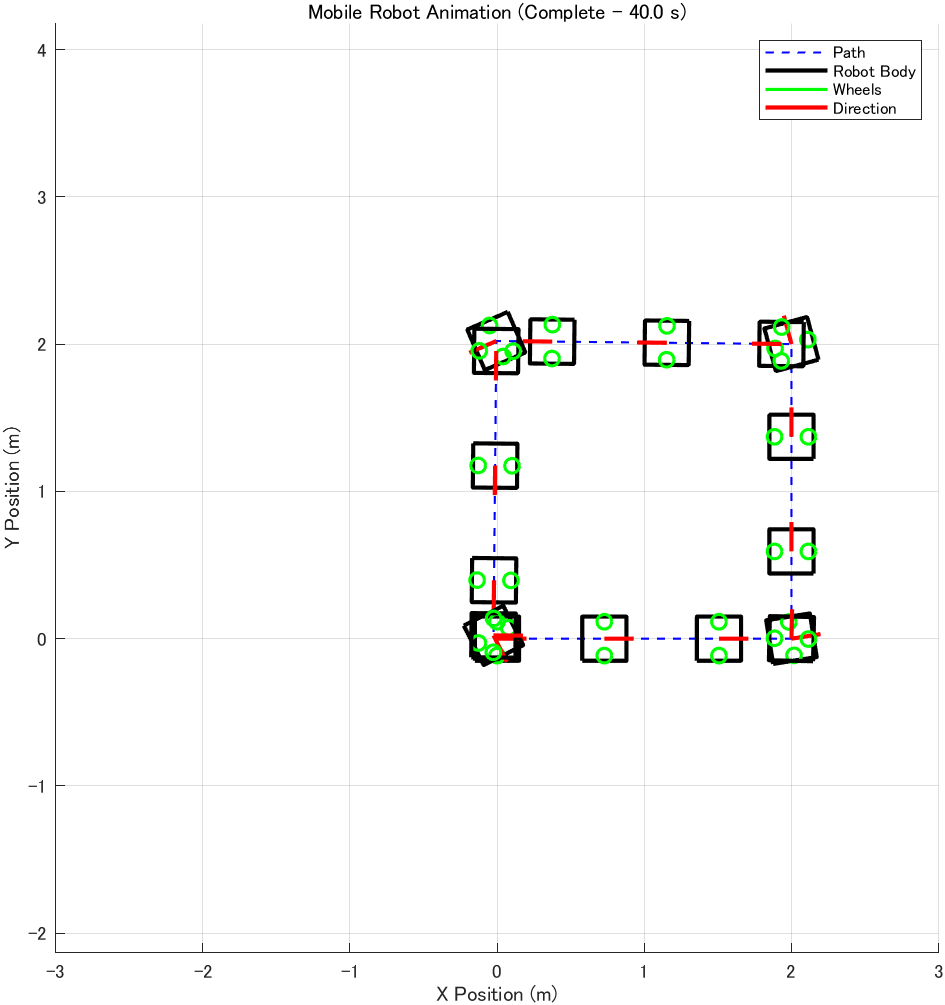
\includegraphics[width=0.6\linewidth]{242C2016_NaoOkumura_3_5_a.eps} % 拡張子付きOK(dvipdfmx前提)
\end{figure}

\begin{figure}[H] % Hで「ここに出せ」と指定(\usepackage{here}が必要)
  \centering
  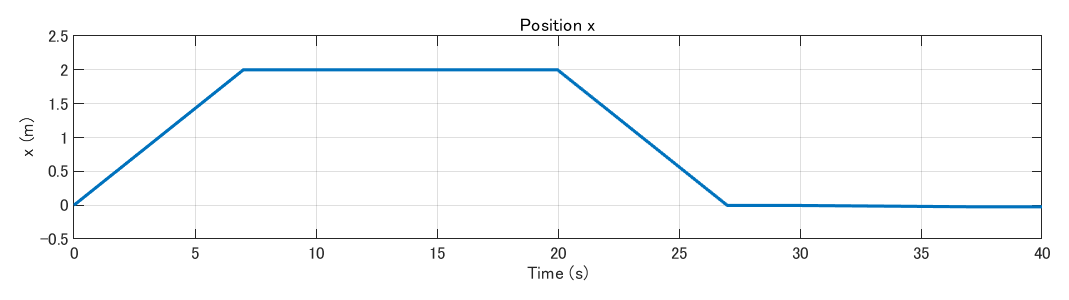
\includegraphics[width=0.6\linewidth]{242C2016_NaoOkumura_3_5_b.eps} % 拡張子付きOK(dvipdfmx前提)
\end{figure}

\begin{figure}[H] % Hで「ここに出せ」と指定(\usepackage{here}が必要)
  \centering
  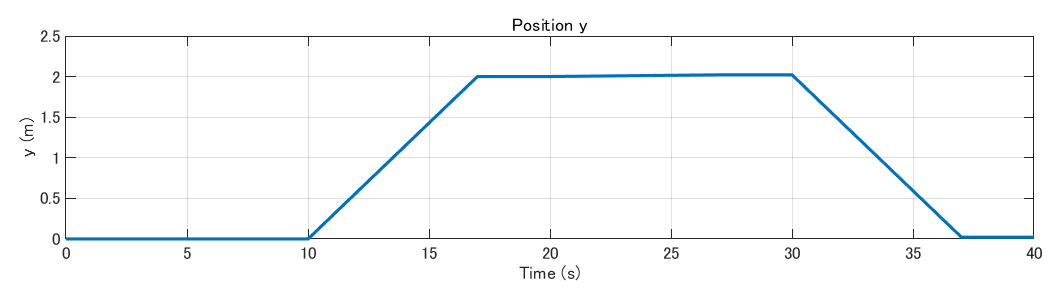
\includegraphics[width=0.6\linewidth]{242C2016_NaoOkumura_3_5_c.eps} % 拡張子付きOK(dvipdfmx前提)
\end{figure}

\begin{figure}[H] % Hで「ここに出せ」と指定(\usepackage{here}が必要)
  \centering
  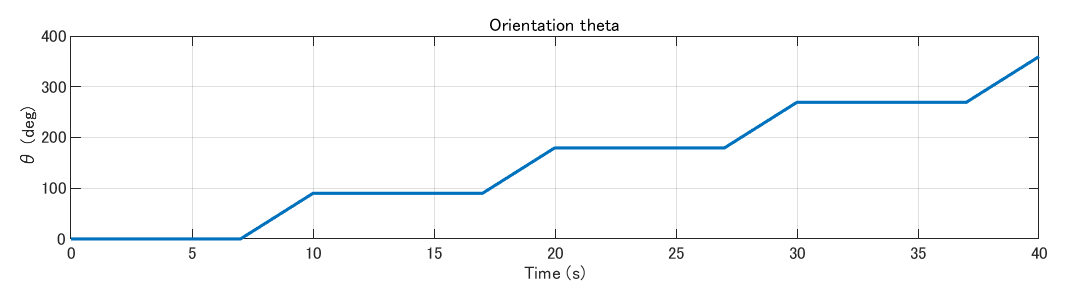
\includegraphics[width=0.6\linewidth]{242C2016_NaoOkumura_3_5_d.eps} % 拡張子付きOK(dvipdfmx前提)
\end{figure}

\chapter{参考文献}

- テキスト(第3章)

\end{document}